\section{evaluation}
\label{sec:evaluation}

To evaluate the performance of LCD-GDP, we conducted experiments with
two devices: one Nexus 4 smartphone and one Samsung Galaxy 10.1-inch
tablet.  We set up video calls between the two devices in the same LAN in order to minimize the impact of the network and we measure the
real power consumption using the Monsoon power monitor~\cite{monsoon}.
In addition, we examine if video call quality has been affected by our
LCD-GDP scheme.

 
\subsection{Power Consumption}
  
%\setlength{\belowcaptionskip}{-10pt}

\begin{figure}[t]
  \begin{center}
    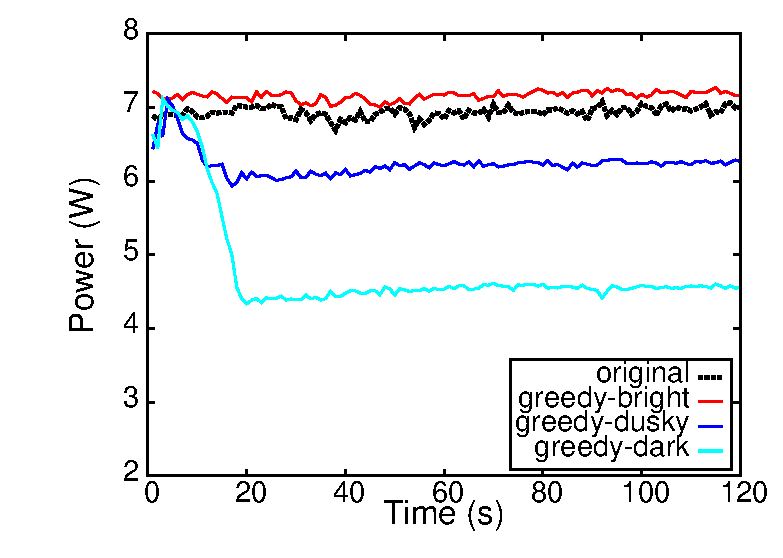
\includegraphics[scale=.6]{./figures/power.eps}
    \caption{Power consumption of the Samsung tablet during real-time video communication under different scenes.}
    \label{fig:power}
  \end{center}
  %\vspace{-3em}
\end{figure}


We measure the power consumption under scenes with different levels of
brightness.  These scenes are tagged with {\it bright}, {\it dusky}
and {\it dark}.  Under the {\it bright} scene, the maximum pixel
luminance of frames is close to 255, which leaves our LCD-GDP scheme
very little space for backlight scaling.  Under the {\it dusky} and
{\it dark} scenes, with smaller maximum luminance value (about 190 and
107, respectively), we can save more power by dimming the backlight
and maintain the observed brightness via luminance compensation.  We
compare the power consumption of our LCD-GDP scheme under different
scenes with the power consumption of the original version of WebRTC
app.  The results are shown in Figure~\ref{fig:power}.  Since the
power consumption of the original WebRTC app under different scenes is
almost the same, we only plot the result under bright environment in
this figure, which is $6.935$ watts on average.  This value is
considered as the baseline.  Under the same {\it bright} scene, and
the power consumption of our LCD-GDP is $7.160$ watts, slightly higher
than the baseline.  This is because extra modules are integrated into
the system, consuming more power, while the backlight is never dimmed
throughout the conversation.  In the {\it dusky} and {\it dark} scene
experiments, the backlight intensity is gradually dimmed by the greedy
algorithm, reducing the power consumption shown as the beginning
descendent gradient.  As a result, only $6.235$ watts and $4.783$
watts power is consumed on average, saving $12.92\%$ and $33.20\%$
power, respectively.
%

\subsection{Video Quality}

We next examine the quality of video calls made under our LCD-GDP
scheme. We focus four metrics frames per second (FPS), peak
signal to noise ratio (PSNR), structural similarity (SSIM), and user-perceived video call latency.
We compare our scheme with the original WebRTC app.

\noindent{\bf Frame Rate.} 
To measure the number of frames that are captured, encoded at the
sender side and decoded and rendered at the receiver side, we use the
statistics reported by the WebRTC app directly. We find that at the
sender side, the number of frames that are encoded varies
significantly if there are moving objects.  The frame rate reaches the
highest value when the frame content is a static scene.  Since our
scheme is agnostic to frame content, we only consider static scene in
our experiments.  This allows us to evaluate our scheme during video
call with a large number of frames per second.  We expect if our scheme
will not impact the video call with higher FPS, it will not impact the
calls with lower FPS either.  We set the resolution of captured video
to $640\times 480$ and measured the FPS under scenes with different
brightness.  Note that in the WebRTC app where we incorporated our
LCD-GDP scheme, the frame rate of generation is limited to $30$ FPS
and at most $15$ frames are rendered per second. In each experiment,
the video call lasted at least $5$ minutes. 
During the video call, the FPS metric is recorded every second. 
Then we report the statistical results of the FPS in different stages for the
video streaming originating from the Nexus smartphone to the Samsung tablet.



\begin{table}[t]
  \small
  \centering
  \caption{FPS of video stream originating from Nexus 4 smartphone to
    Samsung tablet.}
	\vspace{0.5em}
  \label{tab:fps}
  %% fps input | fps sent | fps received | fps decoded | fps output | sent bitrate | receive bitrate
  \begin{tabular}{|c||c|c||c|c||c|c|} %lcr
    \hline
%    & \multicolumn{6}{|c|}{FPS} \\ \hline
    & \multicolumn{2}{|c||}{Input} & \multicolumn{2}{|c||}{Sent}
    & \multicolumn{2}{|c|}{Output}
    \\ \hline
    & $E$ & $\delta$ & $E$ & $\delta$ & $E$ & $\delta$ \\ \hline
    \multicolumn{7}{|c|}{Bright scenario} \\ \hline
    Original App & $23.78$ & $1.66$ & $19.09$ & $2.81$ & $13.91$ & $4.41$ 
    \\ \hline
    LCD-GDP & $23.99$ & $1.18$ & $18.79$ & $3.06$ & $13.60$ & $3.17$
    \\ \hline
    \multicolumn{7}{|c|}{Dark scenario} \\ \hline
    Original App & $8.02$ & $1.37$ & $8.00$ & $0.42$ & $4.85$ & $0.72$ \\ \hline
    LCD-GDP & $7.85$ & $0.48$ & $8.00$ & $0.18$ & $4.96$ & $0.53$ \\ \hline
    %% & \multicolumn{2}{inputfps} & \multicolumn{2}{sentfps} & \multicolumn{2}{outputfps} & sentbitrate & recvbitrate \\ \hline
  \end{tabular}
  %\vspace{-18pt}  
\end{table}


Table~\ref{tab:fps} shows the frame rate of the video stream originated from the Nexus 4 smartphone 
in different stages. The {\it Input} column indicates the rate of frames captured at the camera. 
The {\it Sent} column indicates the frame rate of the encoded video stream.
This stream is sent over the network and decoded at the receiver side.
The final rendered frame rate is shown in the {\it Output} column. 
$E$ stands for the
expectation of the result and $\delta$ is the corresponding standard
deviation. The table shows that FPS is always lower in the dark scenario
even in the original scheme. We find this frame rate degradation
is due to the specific implementation of the original WebRTC app. Comparing these two
extreme cases in the lowest FPS and the highest FPS,  we find there is no degradation of video quality in terms of FPS.

\noindent{\bf Image Fidelity.} 	
Fidelity loss could occur in LCD-GDP for two reasons: (i) the maximum pixel luminance of 
frames increases abruptly, causing the constraint shown in Equation~\cite{eq:distort} be violated;
and (ii) the luminance information piggybacked in the delivered frames is lost due to video
compression or network transmission.
To measure video quality, we calculate the Peak
Signal-to-Noise Ratio (PSNR) and Structural SIMilarity (SSIM) 
between the receiver-observed video stream and the original stream captured at the sender. 
%At the sender side, we record the frames captured by the camera; 
%at the receiver side, we record the frames output from the rendering module.
To align the frames, we insert a black frame into the streaming every $10$ 
frames as the anchor. Then we record all the frames on both sides. 
We only compare the frames between two anchor frames if there 
are exactly $10$ frames recorded on both sides. 
The results are shown in the Table~\ref{tab:distortion}.

Using the original WebRTC app under Dusky Scene, for example, the PSNR and SSIM between 
the rendered frame and the original captured frame is 41.79 and 0.98, respectively. 
The difference is caused by video compression as expected. We use this value as baseline
and see if using the greedy algorithm causes more fidelity loss. 
The result show that the PSNR and SSIM of LCD-GDP under the same scene has the same
value of 41.79, indicating video quality is not affected.
Under the Bright Scene and the Dark Scene, the PSNR is slightly decreased using LCD-GDP.
However, the PSNR values are still above 40 dB, indicating there is very little distortion.

%Potentially, with LCD-GDP, there are two possible reasons that may
%cause the received frames to lose image fidelity: 1) the luminance
%information piggybacked in the delivered frames is lost due to video
%compression or network transmission, 2) the maximum luminance of
%consecutive frames increases abruptly. To investigate this potential
%quality loss, we measured the received video quality using both Peak
%Signal-to-Noise Ratio (PSNR) and Structure SIMilarity (SSIM). To align
%the frames, a black frame is inserted into the streaming every $10$
%frames as the anchor. Then we recorded all the frames on both
%sides. We only compare the frames between two anchor frames if there
%are exact $10$ frames recorded on both sides.  The resemblance of the
%frames is measured in the case of  original WebRTC implementation
%("Original" in the table), using dynamic programming for luminance
%adjustment ("DP" in the table), and our greedy algorithm ("Greedy" in
%the table).  We conducted this experiments under the same scenes where
%we performed the power consumption experiment. The length of the
%videos measured in  this experiment are all $3$ minutes. The results
%are shown in the Table~\ref{tab:distortion}.

%\begin{table}[t]
%  \small
%  \centering
%  \caption{Image fidelity}
%  
%  \begin{tabular}{|c|c|c|c|c|c|c|}
%    \hline
%    & \multicolumn{2}{|c|}{Original} & \multicolumn{2}{|c|}{DP} & \multicolumn{2}{|c|}{Greedy} \\ \hline
%    & $E$ & $\delta$ & $E$ & $\delta$ & $E$ & $\delta$ \\ \hline
%    \multicolumn{7}{|c|}{bright} \\ \hline
%    PSNR & 41.89 & 4.85 & 41.57 & 4.96 & 41.79 & 4.85 \\ \hline
%    SSIM & 0.98 & 0.01 & 0.98 & 0.01 & 0.98 & 0.01 \\ \hline
%    \multicolumn{7}{|c|}{dusky} \\ \hline
%    PSNR & 41.79 & 4.85 & 41.57 & 4.96 & 41.79 & 4.85 \\ \hline
%    SSIM & 0.98 & 0.01 & 0.98 & 0.01 & 0.98 & 0.01 \\ \hline
%    \multicolumn{7}{|c|}{dark} \\ \hline
%    PSNR & 44.86 & 6.88 & 41.63 & 9.62 & 41.63 & 9.78 \\ \hline
%    SSIM & 0.97 & 0.01 & 0.97 & 0.01 & 0.97 & 0.01 \\ \hline
%  \end{tabular}
%  \label{tab:distortion}
%\end{table}

%% In this table, we show the expectation and standard deviation in both
%% PSNR and SSIM respectively.  From the results of PSNR and SSIM, the
%% similarity of frames between sender and receiver stays almost same in
%% bright and dusky scenes. In the dark scenes, our scheme undermine the
%% resemblance of the images in PSNR. The reason is in the dark
%% environment, the frames transmitted have lower contrast. The luminance
%% information stored in the frames will lose in higher probability other
%% than the previous two cases. But the PSNR result of $41.63$ are still
%% a good rendered quality. So we can conclude that little distortion is
%% introduced into the video conferencing by applying our LCD-GDP.


\begin{table}[t]
	\small
	\centering
	\caption{PSNR (dB) and SSIM between the rendered video stream and the original captured frame.}
	\vspace{0.5em}
	\begin{tabular}{|c||c|c||c|c|}
		\hline
		& \multicolumn{2}{|c||}{Original WebRTC App} & \multicolumn{2}{|c|}{LCD-GDP} \\ \hline
		& $E$ & $\delta$ & $E$ & $\delta$ \\ \hline
		\multicolumn{5}{|c|}{Bright Scene} \\ \hline
		PSNR & 41.89 & 4.85 & 41.79 & 4.85 \\ \hline
		SSIM & 0.98 & 0.01  & 0.98 & 0.01 \\ \hline
		\multicolumn{5}{|c|}{Dusky Scene} \\ \hline
		PSNR & 41.79 & 4.85  & 41.79 & 4.85 \\ \hline
		SSIM & 0.98 & 0.01  & 0.98 & 0.01 \\ \hline
		\multicolumn{5}{|c|}{Dark Scene} \\ \hline
		PSNR & 44.86 & 6.88  & 41.63 & 9.78 \\ \hline
		SSIM & 0.97 & 0.01  & 0.97 & 0.01 \\ \hline
	\end{tabular}
	\label{tab:distortion}
        %\vspace{-18pt}  
\end{table}


%From the table, we can see in the dusky setting, the PSNR for
%original, DP, and Greedy is $41.89\pm4.85$, $41.57\pm4.96$ and
%$41.79\pm4.85$ respectively. The DP and the Greedy algorithm both make
%no promotion on this metric. The corresponding SSIM values are all
%$0.98\pm0.01$, confirming that there is no difference perceived by the
%user. Similar results are observed in the case of bright and dark
%cases.


\noindent{\bf User-perceived Video Latency.} 
We also measure the user-perceived video call delay.
To minimize the impact of wide area network dynamics, 
we conduct the experiments in the same local area network (LAN).
%At last, the communication latency is also measured between these two machines. 
To measure the end-to-end delay, 
we place the camera on the mobile device in front of a stop watch
and compare the timestamps rendered on two devices using the method proposed by Yu et al.~\cite{6848080}. 
In the original WebRTC app, we find the average latency is $261$ milliseconds 
during the video call. When the LCD-GDP scheme is applied, the average latency
is increased to $302$ milliseconds, indicating only about $40$ milliseconds delay are
introduced due to the additional processing. 


%% \begin{table}[h]
%%   \centering
%%   \caption{video latency}
%%   \label{tab:latency}
%%   \begin{tabular}{|c|c|}
%%     \hline
%%     & latency (ms) \\ \hline
%%     Original & 261 \\ \hline
%%     Greedy & 302 \\ \hline
%%   \end{tabular}
%% \end{table}



%% The Table~\ref{tab:latency} shows the latency measured under different
%% schemes in milliseconds. From the result, the scanning operation and
%% the greedy determination stage introduce minor latency, about tens of
%% milliseconds into video conferencing. 




%% We conducted all the experiments on two devices: one NEXUS 4
%% smartphone and one Samsung Galaxy 10.1-inch tablet. We first examine
%% how much energy can we saved by using the LCD-GDP during the real-time
%% communication. As the
%% additional stages are added into the video conferencing, we then
%% evaluate if our implementation will impact the video streaming
%% quality. Finally we measured if our scheme will introduce distortion
%% into the video calls. 

%% \subsection{Power Consumption}

%% \begin{figure}[t]
%%   \begin{center}
%%   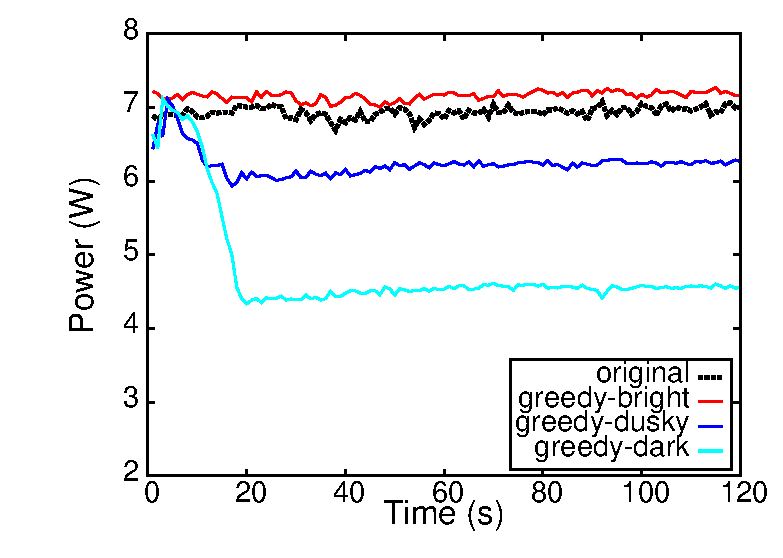
\includegraphics[scale=.5]{./figures/power.eps}
%%   \caption{Power consumption of real-time communication}
%%   \label{fig:power}
%%   \end{center}
%% \end{figure}


%% We measured the power consumption of the real-time
%% communication between these two devices. To evaluate the
%% effect of our system, we test the power consumption under scenes with
%% different levels of brightness. A two-minute conversation is conducted
%% in each experiment. The scenes can be tagged with {\it bright}, {\it
%%   dusky} and {\it dark}, which make backlight level set to $0.99$,
%% $0.75$ and $0.42$ on average in our system. Also we measured the power
%% consumption of the original version of WebRTC app. The results are
%% plot on figure~\ref{fig:power}. The x-axis is the time in seconds, and
%% the y-axis is the power consumption in walts. In this figure, power
%% consumption of the original WebRTC app under different scenes is
%% almost in same level so only the result under bright environment is
%% plot, which is $6.935$ walts on average. This value is considered as
%% the baseline and the power consumption of our system is found slightly
%% higher than it, which is $7.160$ walts. The reason is that extra
%% modules are integrated into the system but the backlight has never
%% been dimmed across the conversation. In the dusky and dark case,
%% $6.235$ ($12.92\%$) walts and $4.783$ ($33.20\%$) walts is consumed on
%% average by dimming the backlight intensity. The beginning descendent
%% gradient shows the process of the greedy algorithm dimming the
%% backlight intensity.


%% \subsection{Video quality}
%% In worrying about our scheme will make the quality of the video calls
%% degrade, we measured the quality metrics in frames per second (fps)
%% and latency. The comparison is made by our greedy scheme and the
%% original version. All the results are reported by the webRTC app
%% itself. 

%% In the measurement, the fps metric varied in great range if moving
%% objects is involved into the frames. The frame rate reached the
%% highest threshold if the frame content is a static scene. Only the
%% static scene is used in our experiment.  We expect if our scheme will
%% not impact the video streaming with higher fps, it won't impact the
%% one with lower fps as well. We measured the fps under scenes with
%% different brightness and the resolution of the video streaming is set as
%% $640$x$480$. In the webRTC app, the frame rate of generation is
%% limited to $30$ fps and at most $15$ frames are rendered per
%% second. At least $5$ minutes streaming is maintained in each
%% experiment. The data is collected from the Samsung tablet. 


%% \begin{table}[h]
%%   \centering
%%   \caption{video frames per second}
%%   \label{tab:fps}
%%   %% fps input | fps sent | fps received | fps decoded | fps output | sent bitrate | receive bitrate
%%   \begin{tabular}{|c|c|c|c|c|c|c|} %lcr
%%     \hline
%%     & \multicolumn{6}{|c|}{fps} \\ \hline
%%     & \multicolumn{2}{|c|}{input} & \multicolumn{2}{|c|}{sent}
%%     & \multicolumn{2}{|c|}{output}
%%     \\ \hline
%%     & $E$ & $\delta$ & $E$ & $\delta$ & $E$ & $\delta$ \\ \hline
%%     \multicolumn{7}{|c|}{bright scenario} \\ \hline
%%     original & $23.78$ & $1.66$ & $19.09$ & $2.81$ & $13.91$ & $4.41$ 
%%     \\ \hline
%%     greedy & $23.99$ & $1.18$ & $18.79$ & $3.06$ & $13.60$ & $3.17$
%%     \\ \hline
%%     \multicolumn{7}{|c|}{dark scenario} \\ \hline
%%     original & $8.02$ & $1.37$ & $8.00$ & $0.42$ & $4.85$ & $0.72$ \\ \hline
%%     greedy & $7.85$ & $0.48$ & $8.00$ & $0.18$ & $4.96$ & $0.53$ \\ \hline
%%     %% & \multicolumn{2}{inputfps} & \multicolumn{2}{sentfps} & \multicolumn{2}{outputfps} & sentbitrate & recvbitrate \\ \hline
%%   \end{tabular}
  
%% \end{table}


%% In the Table~\ref{tab:fps}, we show the fps of the video in different
%% stages. The {\it input} tag means the frame generation rate of the
%% capturer. {\it sent} and {\it output} means the network sent rate and
%% final rendering frame rate respectively. $E$ stands for the
%% expectation of the result and $\delta$ is the corresponding standard
%% deviation. From this table, fps is always lower in the dark scenario
%% even in the original scheme. We can conclude this quality degradation
%% is due to the specific implementation of this app. Comparing these two
%% extreme cases in the lowest fps and the highest fps, there is no
%% degradation of the video quality in fps is found. 

%% The communication latency is also measured between these two
%% machine. We use the method proposed in~\cite{yu2014can}. In the
%% original version, $261$ milliseconds of latency on average is found
%% during the video call. When applying the LCD-GDP, the average latency
%% increases to $302$ milliseconds. Only $40$ milliseconds are
%% introduced. 


%% To evaluate the power consumption of our system, we setup the devices
%% under scenes with different brightness and the power consumption of
%% the tablet is measured by the power monitor. The results are shown in
%% ~\ref{tab:power_consumption}.
 
%% installed the original version WebRTC app and an upgraded version
%% equipped with our dynamic programming scheme. When these two devices
%% connected to each other, we put them under different environments to
%% evaluate if our scheme could outperform the original version. Two
%% extreme environments were selected purposely. One was an extreme
%% bright environment that our scheme didn't work any more. Under the
%% other environment, which is an extreme dark case, the backlight could
%% always be scaled to the lowest threshold($0.4$).
%% We measured the power
%% consumption of the tablets in all of these cases and the results are
%% shown in ~\ref{tab:power_consumption}.


%% \begin{table}[h]
%%   \centering
%%   \caption{power consumption}
%%   \label{tab:power_consumption}
%%   %% device | dark | bright |
%%   \begin{tabular}{|c|c|c|c|c|} %lcr
%%     \hline
%%     & \multicolumn{2}{|c|}{SAMSUNG(dark)} & \multicolumn{2}{|c|}{SAMSUNG(bright)} \\ \hline
%%     & no-adaption & with adaption & no-adaption & with adaption \\ \hline
%%     NEXUS(dark) & $\sim{6250}$ mW & $\sim{3810}$ mW & $\sim{6900}$ mW & $\sim{4150}$ mW  \\ \hline
%%     NEXUS(bright) & $\sim{6500}$ mW & $\sim{6400}$ mW & $\sim{7250}$ mW & $\sim{6800}$ mW \\ \hline
%%   \end{tabular}
  
%% \end{table}

%% From the table, we found that the original version WebRTC app consumed
%% similar power, which was from $6250$ mA to $7250$ mA, under different
%% environments. The slight difference are caused by the mutable fps. The
%% WebRTC app actively reduces the fps if it detects that the environment
%% gets dark. So the power consumption was found lowest when both the
%% devices were put in the dark environment. The most observable power
%% savings were found in the case that the NEXUS was put in the dark
%% environment. The dimmed frames sent by the NEXUS help the tablet take
%% advantage of the luminance compensation technique.  Notice that
%% although our scheme outperformed the original version in the both
%% bright case. This power reduction comes from the lower fps. The
%% dynamic programming algorithm, holding too many frames before
%% delivering them to the rendering module, will definitely degrade the
%% video quality.

%% \begin{table}[h]
%%   \centering
%%   \caption{power consumption}
%%   \label{tab:power_consumption}
%%   %% device | dark | bright |
%%   \begin{tabular}{|c|c|c|c|c|} %lcr
%%     \hline
%%     & \multicolumn{2}{|c|}{SAMSUNG(dark)} & \multicolumn{2}{|c|}{SAMSUNG(bright)} \\ \hline
%%     & no-adaption & with adaption & no-adaption & with adaption \\ \hline
%%     NEXUS(dark) & $\sim{6250}$ mW & $\sim{3810}$ mW & $\sim{6900}$ mW & $\sim{4150}$ mW  \\ \hline
%%     NEXUS(bright) & $\sim{6500}$ mW & $\sim{6400}$ mW & $\sim{7250}$ mW & $\sim{6800}$ mW \\ \hline
%%   \end{tabular}
  
%% \end{table}


%% Expr 1:
%% Comparison between normal case and cases applied our scheme.
%% Prove that our implementation doesn't downgrade the user experience.
%% \begin{itemize}
%%   \item{bitrate}
%%   \item{fps}
%%   \item{maybe others}
%% \end{itemize}

%% Expr 2:
%% Compare the distortion of frames among 1) normal case 2) DP 3)
%% Greedy. store the frames under different brightness. (90\%-100\%,
%% 70\%-80\%, 50\%-60\%).
%% To align the frames. (Can try index the frames in several pixels)
%% \begin{itemize}
%%   \item{PSNR}
%%   \item{SSIM}
%% \end{itemize}



%% The
%% dynamic programming algorithm has to hold enough frames to adjust
%% backlight, so that it can not deliver the frames to the rendering
%% module in time.


%% quality of the video in webRTC is self-adjusted. There are two factors
%% affecting the fps and bitrate: the average luminance of the frames and
%% the content of the frames. The webRTC app intends to reduce the
%% fps/bitrate in darker images. Also the static frames gains higher
%% fps/bitrate other than the frames containing moving objects. To
%% evaluate how much overhead is introduced by our scheme, we only use
%% the static scenario as the test case. We expect if our greedy
%% algorithm won't impair the visual quality of the static scenario,
%% which features higher fps and bitrate, the quality of scenarios
%% containing moving objects will not be damaged as well.



%% \begin{table}[h]
%%   \centering
%%   \caption{video quality}
%%   \label{tab:quality}
%%   %% fps input | fps sent | fps received | fps decoded | fps output | sent bitrate | receive bitrate
%%   \begin{tabular}{|c|c|c|c|c|c|c|c|c|} %lcr
%%     \hline
%%     & \multicolumn{6}{|c|}{fps} & \multicolumn{2}{|c|}{bitrate} \\ \hline
%%     & \multicolumn{2}{|c|}{input} & \multicolumn{2}{|c|}{sent}
%%     & \multicolumn{2}{|c|}{output} & sent & recv
%%     \\ \hline
%%     & $E$ & $\delta$ & $E$ & $\delta$ & $E$ & $\delta$ & & \\ \hline
%%     \multicolumn{9}{|c|}{bright scenario/loopback} \\ \hline
%%     original & $24.67$ & $1.01$ & $22.73$ & $3.59$ & $15.37$ & $2.44$ &
%%     $81076$ & $81344$ \\ \hline
%%     greedy & $24.51$ & $1.06$ & $21.64$ & $2.76$ & $15.19$ & $2.06$ &
%%     $44832$ & $45193$ \\ \hline
%%     \multicolumn{9}{|c|}{bright scenario/remote} \\ \hline
%%     original & $23.78$ & $1.66$ & $19.09$ & $2.81$ & $13.91$ & $4.41$ &
%%     $269094$ & $41583$ \\ \hline
%%     greedy & $23.99$ & $1.18$ & $18.79$ & $3.06$ & $13.60$ & $3.17$ &
%%     $267309$ & $32905$ \\ \hline
%%     \multicolumn{9}{|c|}{dark scenario/loopback} \\ \hline
%%     original & $7.86$ & $0.35$ & $8.00$ & $0.00$ & $7.87$ & $0.40$ &
%%     $168306$ & $168306$ \\ \hline
%%     greedy & $7.88$ & $0.39$ & $8.00$ & $0.05$ & $7.87$ & $0.39$ &
%%     $165936$ & $165936$ \\ \hline
%%     \multicolumn{9}{|c|}{dark scenario/remote} \\ \hline
%%     original & $8.02$ & $1.37$ & $8.00$ & $0.42$ & $4.85$ & $0.72$ &
%%     $462505$ & $924722$ \\ \hline
%%     greedy & $7.85$ & $0.48$ & $8.00$ & $0.18$ & $4.96$ & $0.53$ &
%%     $246837$ & $779452$ \\ \hline
%%     %% & \multicolumn{2}{inputfps} & \multicolumn{2}{sentfps} & \multicolumn{2}{outputfps} & sentbitrate & recvbitrate \\ \hline
%%   \end{tabular}
  
%% \end{table}

%% Two devices are used in this measurement, one Samsung 10.1-inch tablet
%% and one NEXUS 4 smartphone. The data is collected from the tablet. We test the
%% real-time communication in the resolution of $640$x$480$, and set the
%% upperbound of the frames generation by the camera as $30$. Both the
%% dark scenario and the bright scenario are measured. We maintained the
%% communication at least $5$ minutes. We test the {\it loopback} and the
%% {\it remote} respectively. The {\it loopback} means the tablet
%% communicate to itself via network. And the {\it remote} means
%% communication between two devices.
